%% ===== removed from ch3 on 2026-08-13 : fig:sys:links =====
\begin{figure}[tb]
  \centering
  \newcommand{\linkcell}[3]{%
    \begin{subfigure}[b]{#1\linewidth}
      \centering
      \includegraphics[height=32mm]{images/links/link_#2}
      \caption{#3}
    \end{subfigure}}
  \linkcell{.31}{frontrahmen}{Front frame (link 0)}\hfill
  \linkcell{.31}{drehzapfen}{Slew column (link 1)}\hfill
  \linkcell{.31}{ausleger_i}{Inner boom (link 2)}

  \vspace{3mm}
  \linkcell{.31}{ausleger_ii}{Outer boom (link 3)}\hfill
  \linkcell{.31}{messerkopf_schwenk}{Head carrier (link 4)}\hfill
  \linkcell{.31}{messerkopf}{Mowing head (link 5)}

  \vspace{3mm}
  \begin{subfigure}[b]{.31\linewidth}
    \centering
    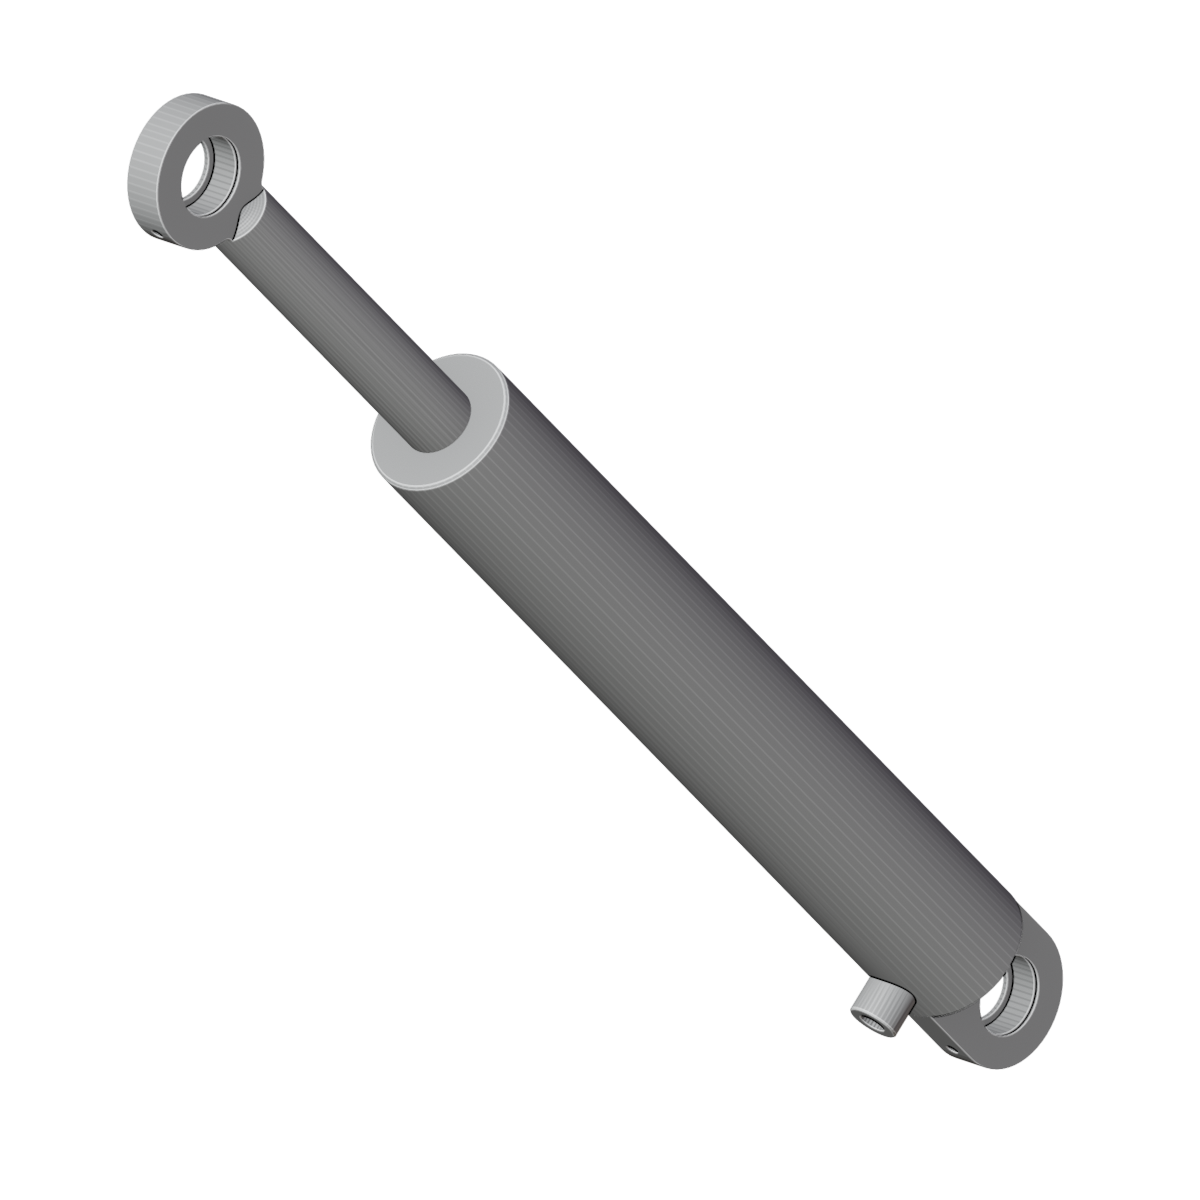
\includegraphics[height=32mm]{images/links/link_cylinder}
    \caption{Cylinder (barrel + rod)}
  \end{subfigure}
  \caption{Catalog of the FME~500 rigid bodies, each rendered
  individually from the URDF geometry in an orthographic view. Links 0--5
  form the serial chain; (g)~shows one of the four hydraulic cylinders as
  the barrel--rod pair that actuates a joint. Renders share the coordinate
  frames, scale, and matte engineering style used throughout the thesis.}
  \label{fig:sys:links}
\end{figure}

%% ===== removed from ch3 on 2026-08-13 : fig:sys:cad =====
\begin{figure}[tb]
  \centering
  \begin{subfigure}[b]{.47\linewidth}
    \centering
    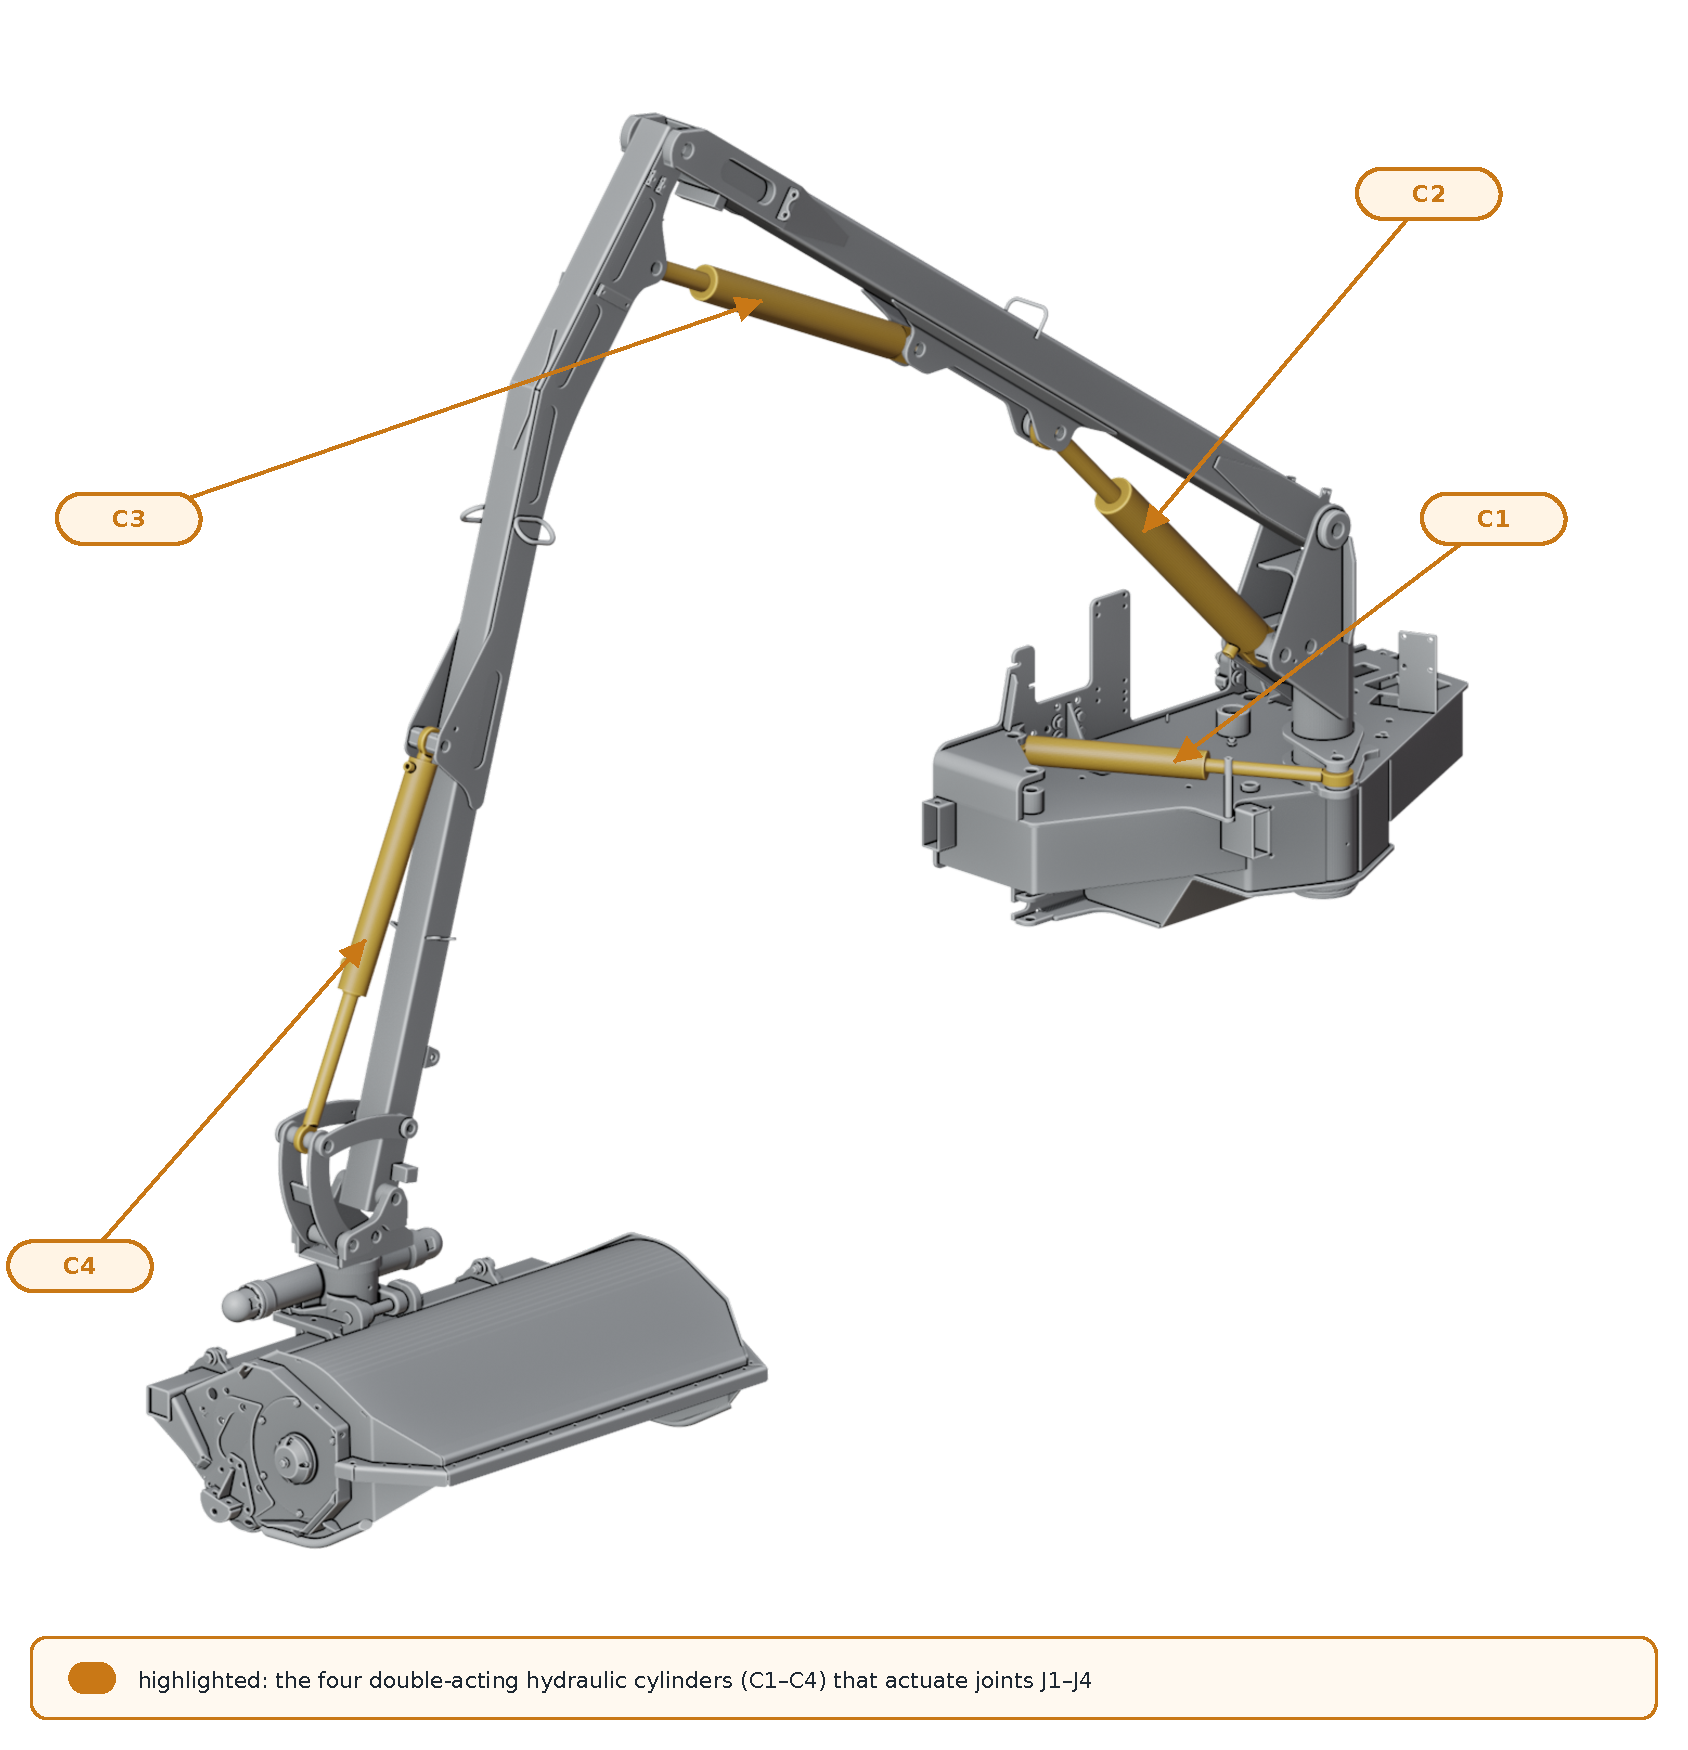
\includegraphics[width=\linewidth]{images/fme500_cad_iso_annot}
    \caption{}
    \label{fig:sys:cad-iso}
  \end{subfigure}
  \hfill
  \begin{subfigure}[b]{.49\linewidth}
    \centering
    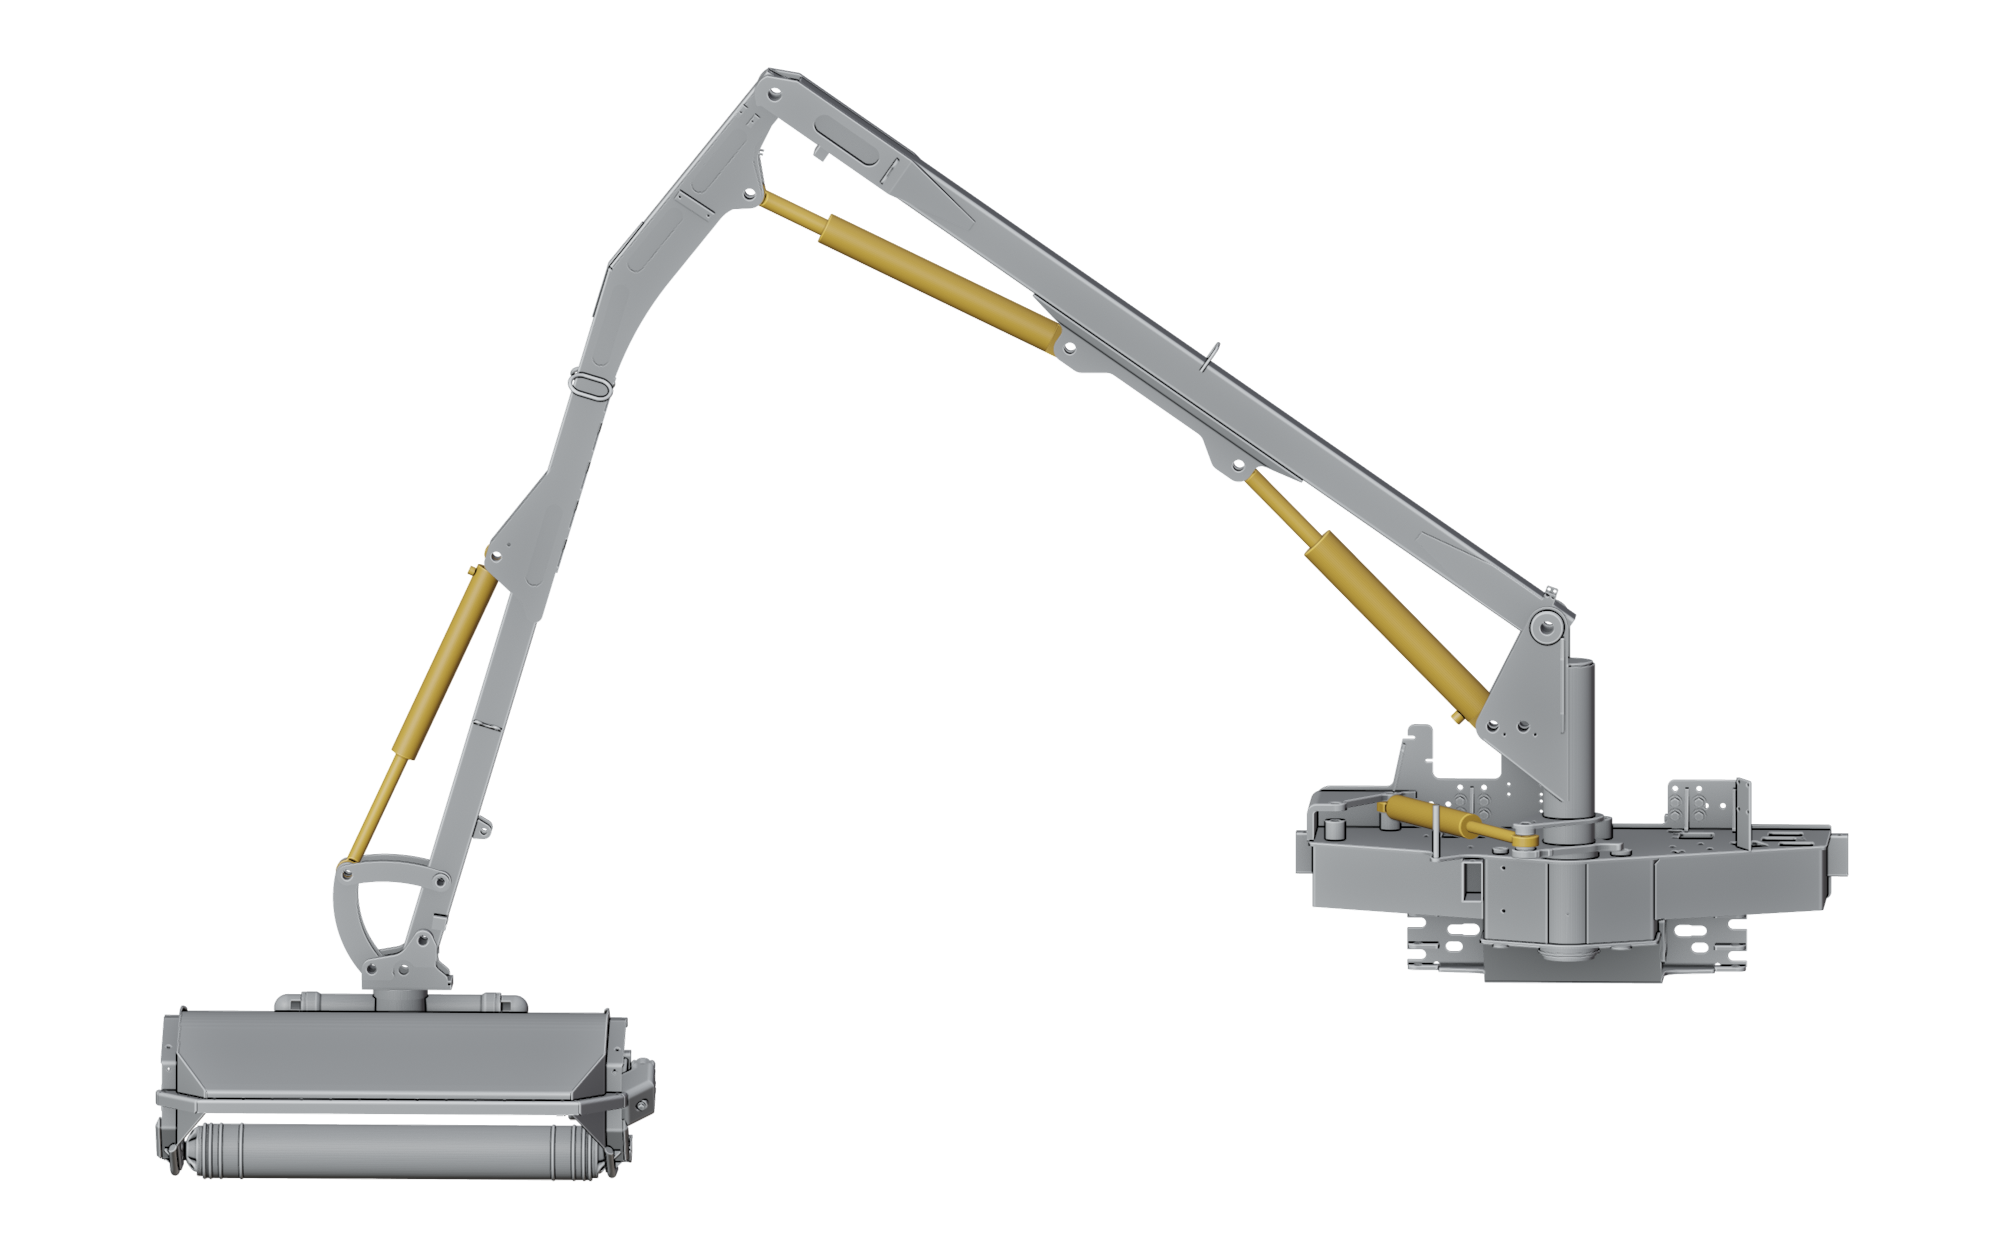
\includegraphics[width=\linewidth]{images/fme500_cad_side}
    \caption{}
    \label{fig:sys:cad-side}
  \end{subfigure}
  \caption{The CAD-derived multibody model of the FME~500 arm, rendered
  from the URDF export used throughout this thesis: (a)~isometric view
  with the four hydraulic cylinders C1--C4 highlighted in orange and
  labeled, (b)~side elevation in the folded zero pose. The swivel links
  of the passive fifth joint connect the head carrier to the flail
  head, and the base frame carries the slew column. The same geometry,
  masses, and inertia tensors drive both the Simscape multibody model
  and the IsaacLab articulation.}
  \label{fig:sys:cad}
\end{figure}

%% ===== removed prose that referenced fig:sys:links =====
%To make the serial chain concrete, Figure~\ref{fig:sys:links} shows the
%individual rigid bodies as they are imported from the URDF, each
%rendered on its own in an orthographic view. Reading outward from the
%vehicle: the \emph{front frame} (link~0) bolts to the Unimog attachment
%plate and carries the slew bearing; the \emph{slew column}
%(\emph{Drehzapfen}, link~1) rotates the whole arm about the vertical
%axis; the \emph{inner} and \emph{outer boom} segments
%(\emph{Ausleger~I} and~\emph{II}, links~2 and~3) are the long
%load-bearing weldments whose asymmetric cross-sections give the
%significant cross-inertia terms noted above; the \emph{head carrier}
%(\emph{Messerkopf-Schwenk}, link~4) with its swivel-link pair sets the
%head orientation; and the \emph{flail mowing head} (link~5) does the
%cutting. The final card in Figure~\ref{fig:sys:links} shows one of the four
%double-acting cylinders as a separate barrel--rod pair, the form in
%which each actuator enters the closed kinematic loop of
%Section~\ref{sec:sys:kinematics}.
%
%

%% ===== ch3 fig:sys:unimog reduced to one panel; original two-panel version =====
\begin{figure}[tb]
  \centering
  \begin{subfigure}[b]{.56\linewidth}
    \centering
    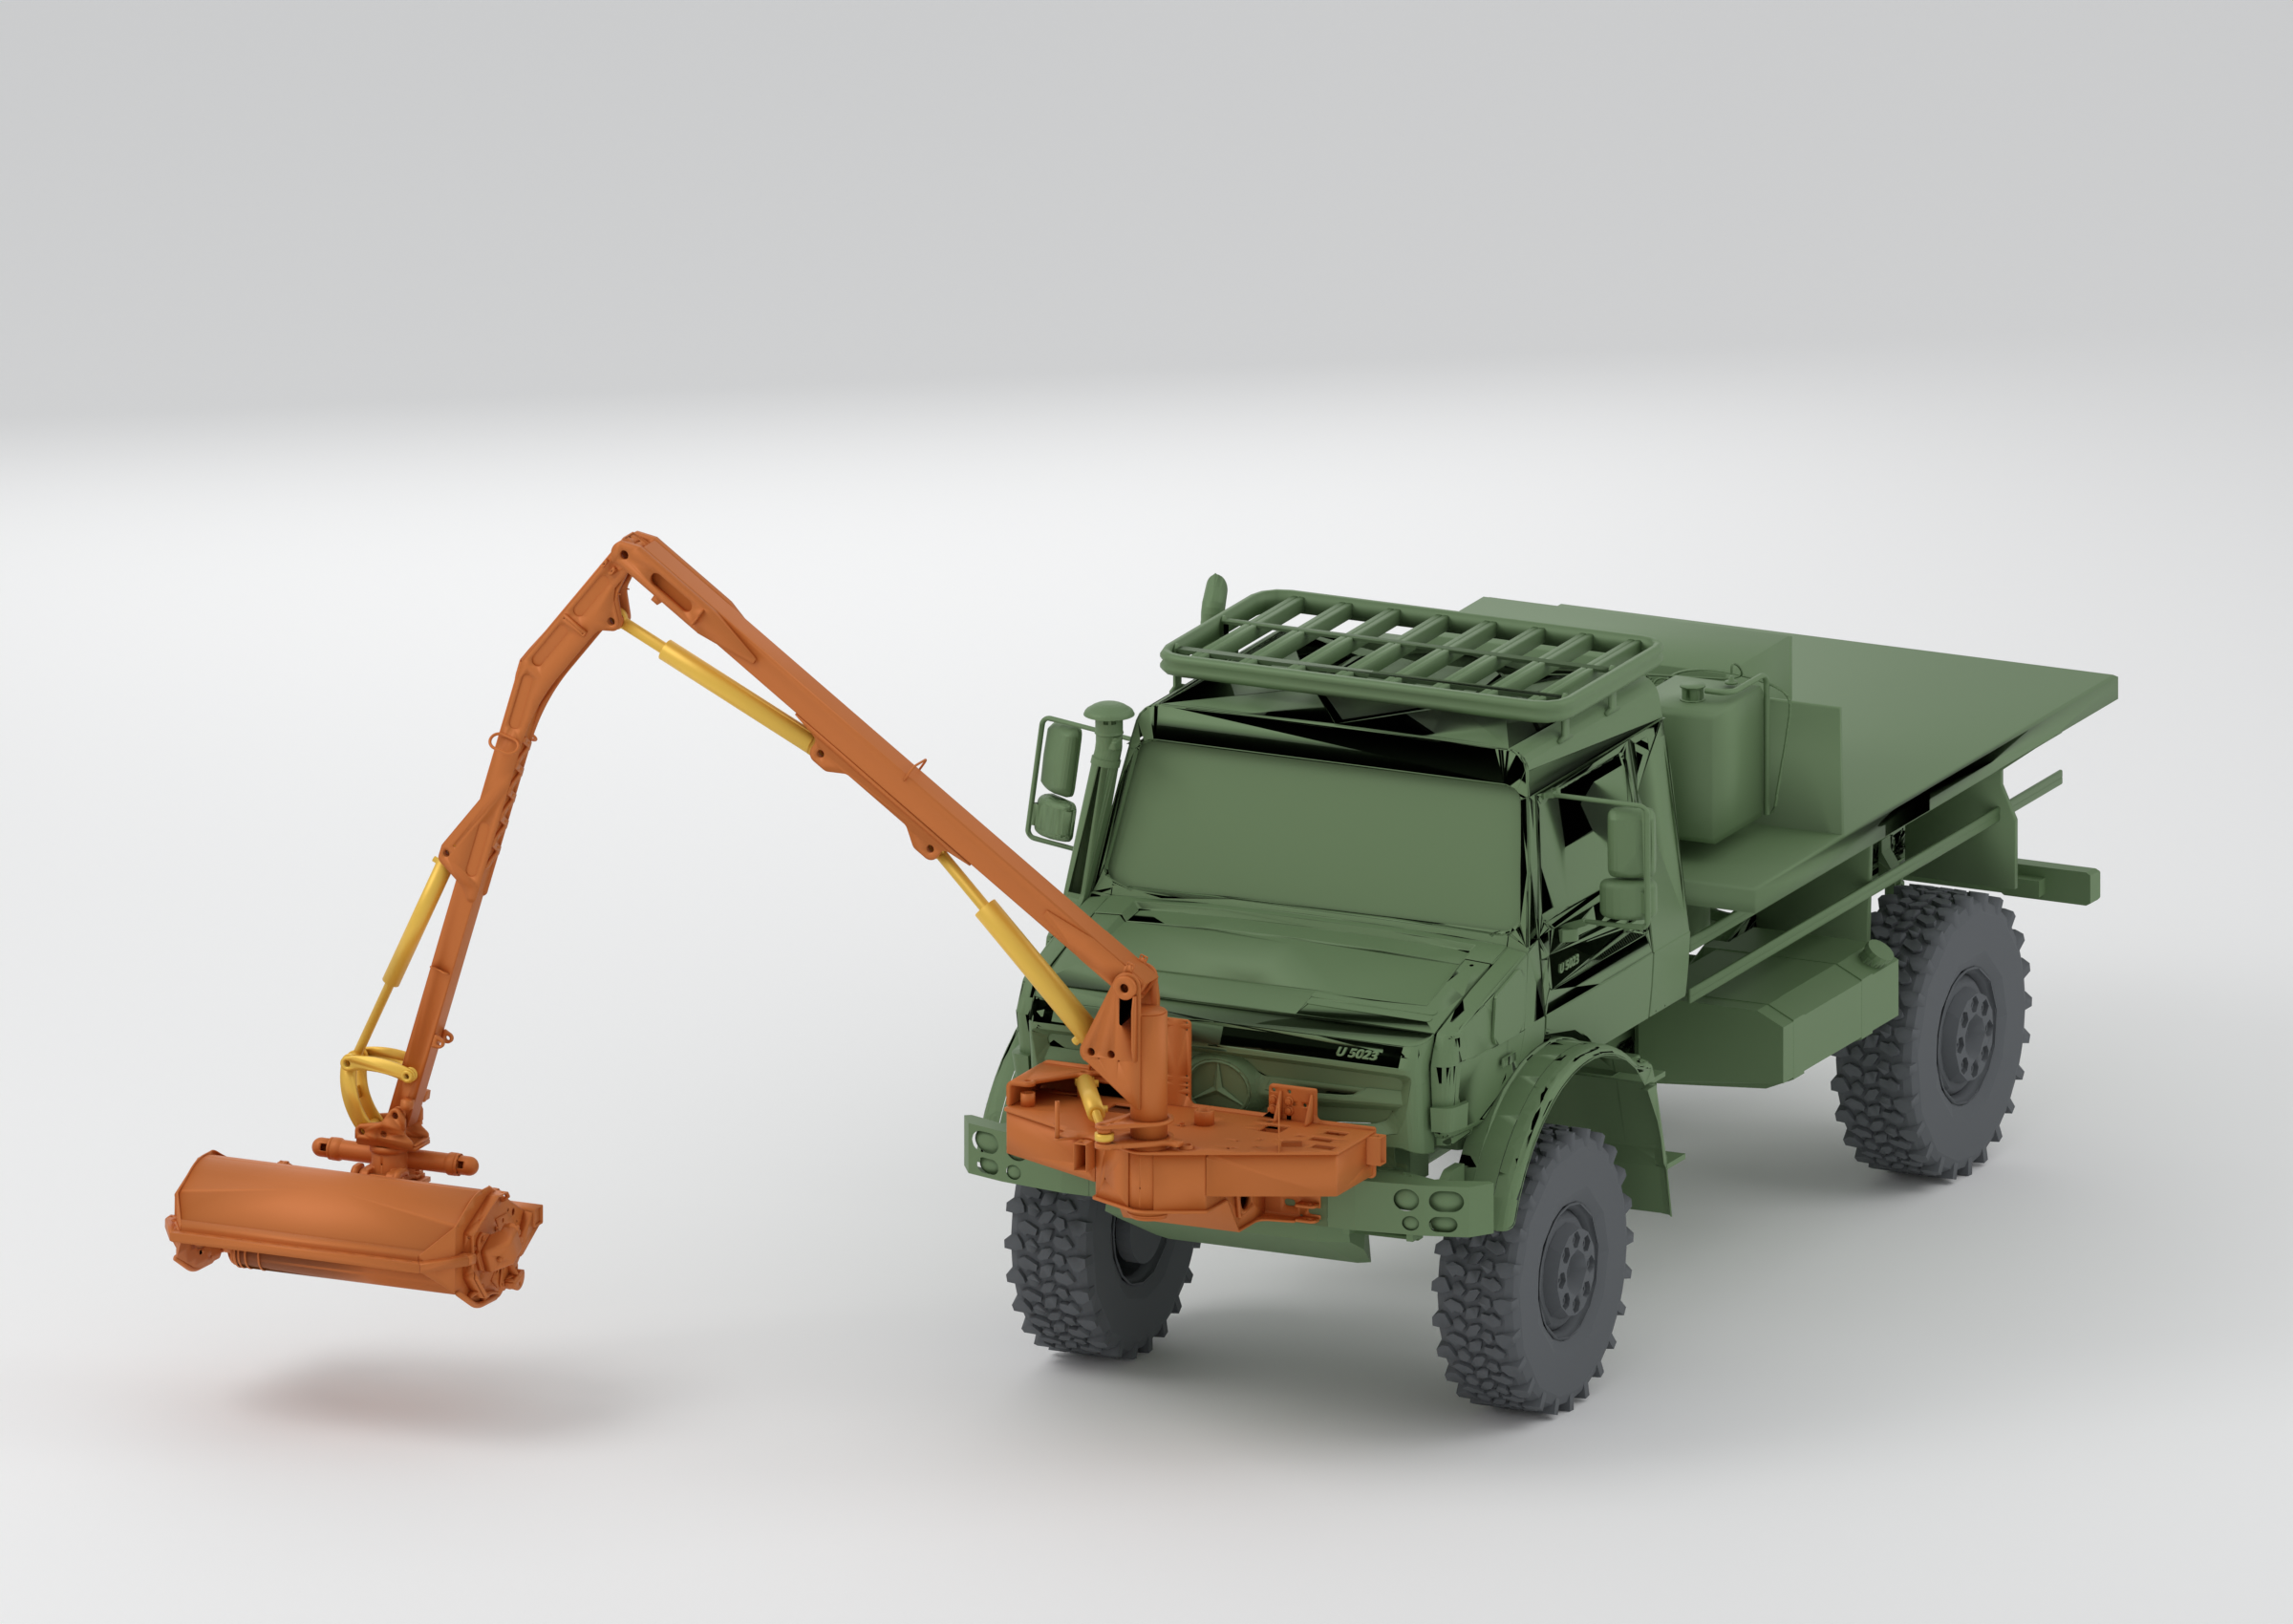
\includegraphics[width=\linewidth]{images/unimog_mulag_iso}
    \caption{}
    \label{fig:sys:unimog-front}
  \end{subfigure}
  \hfill
  \begin{subfigure}[b]{.42\linewidth}
    \centering
    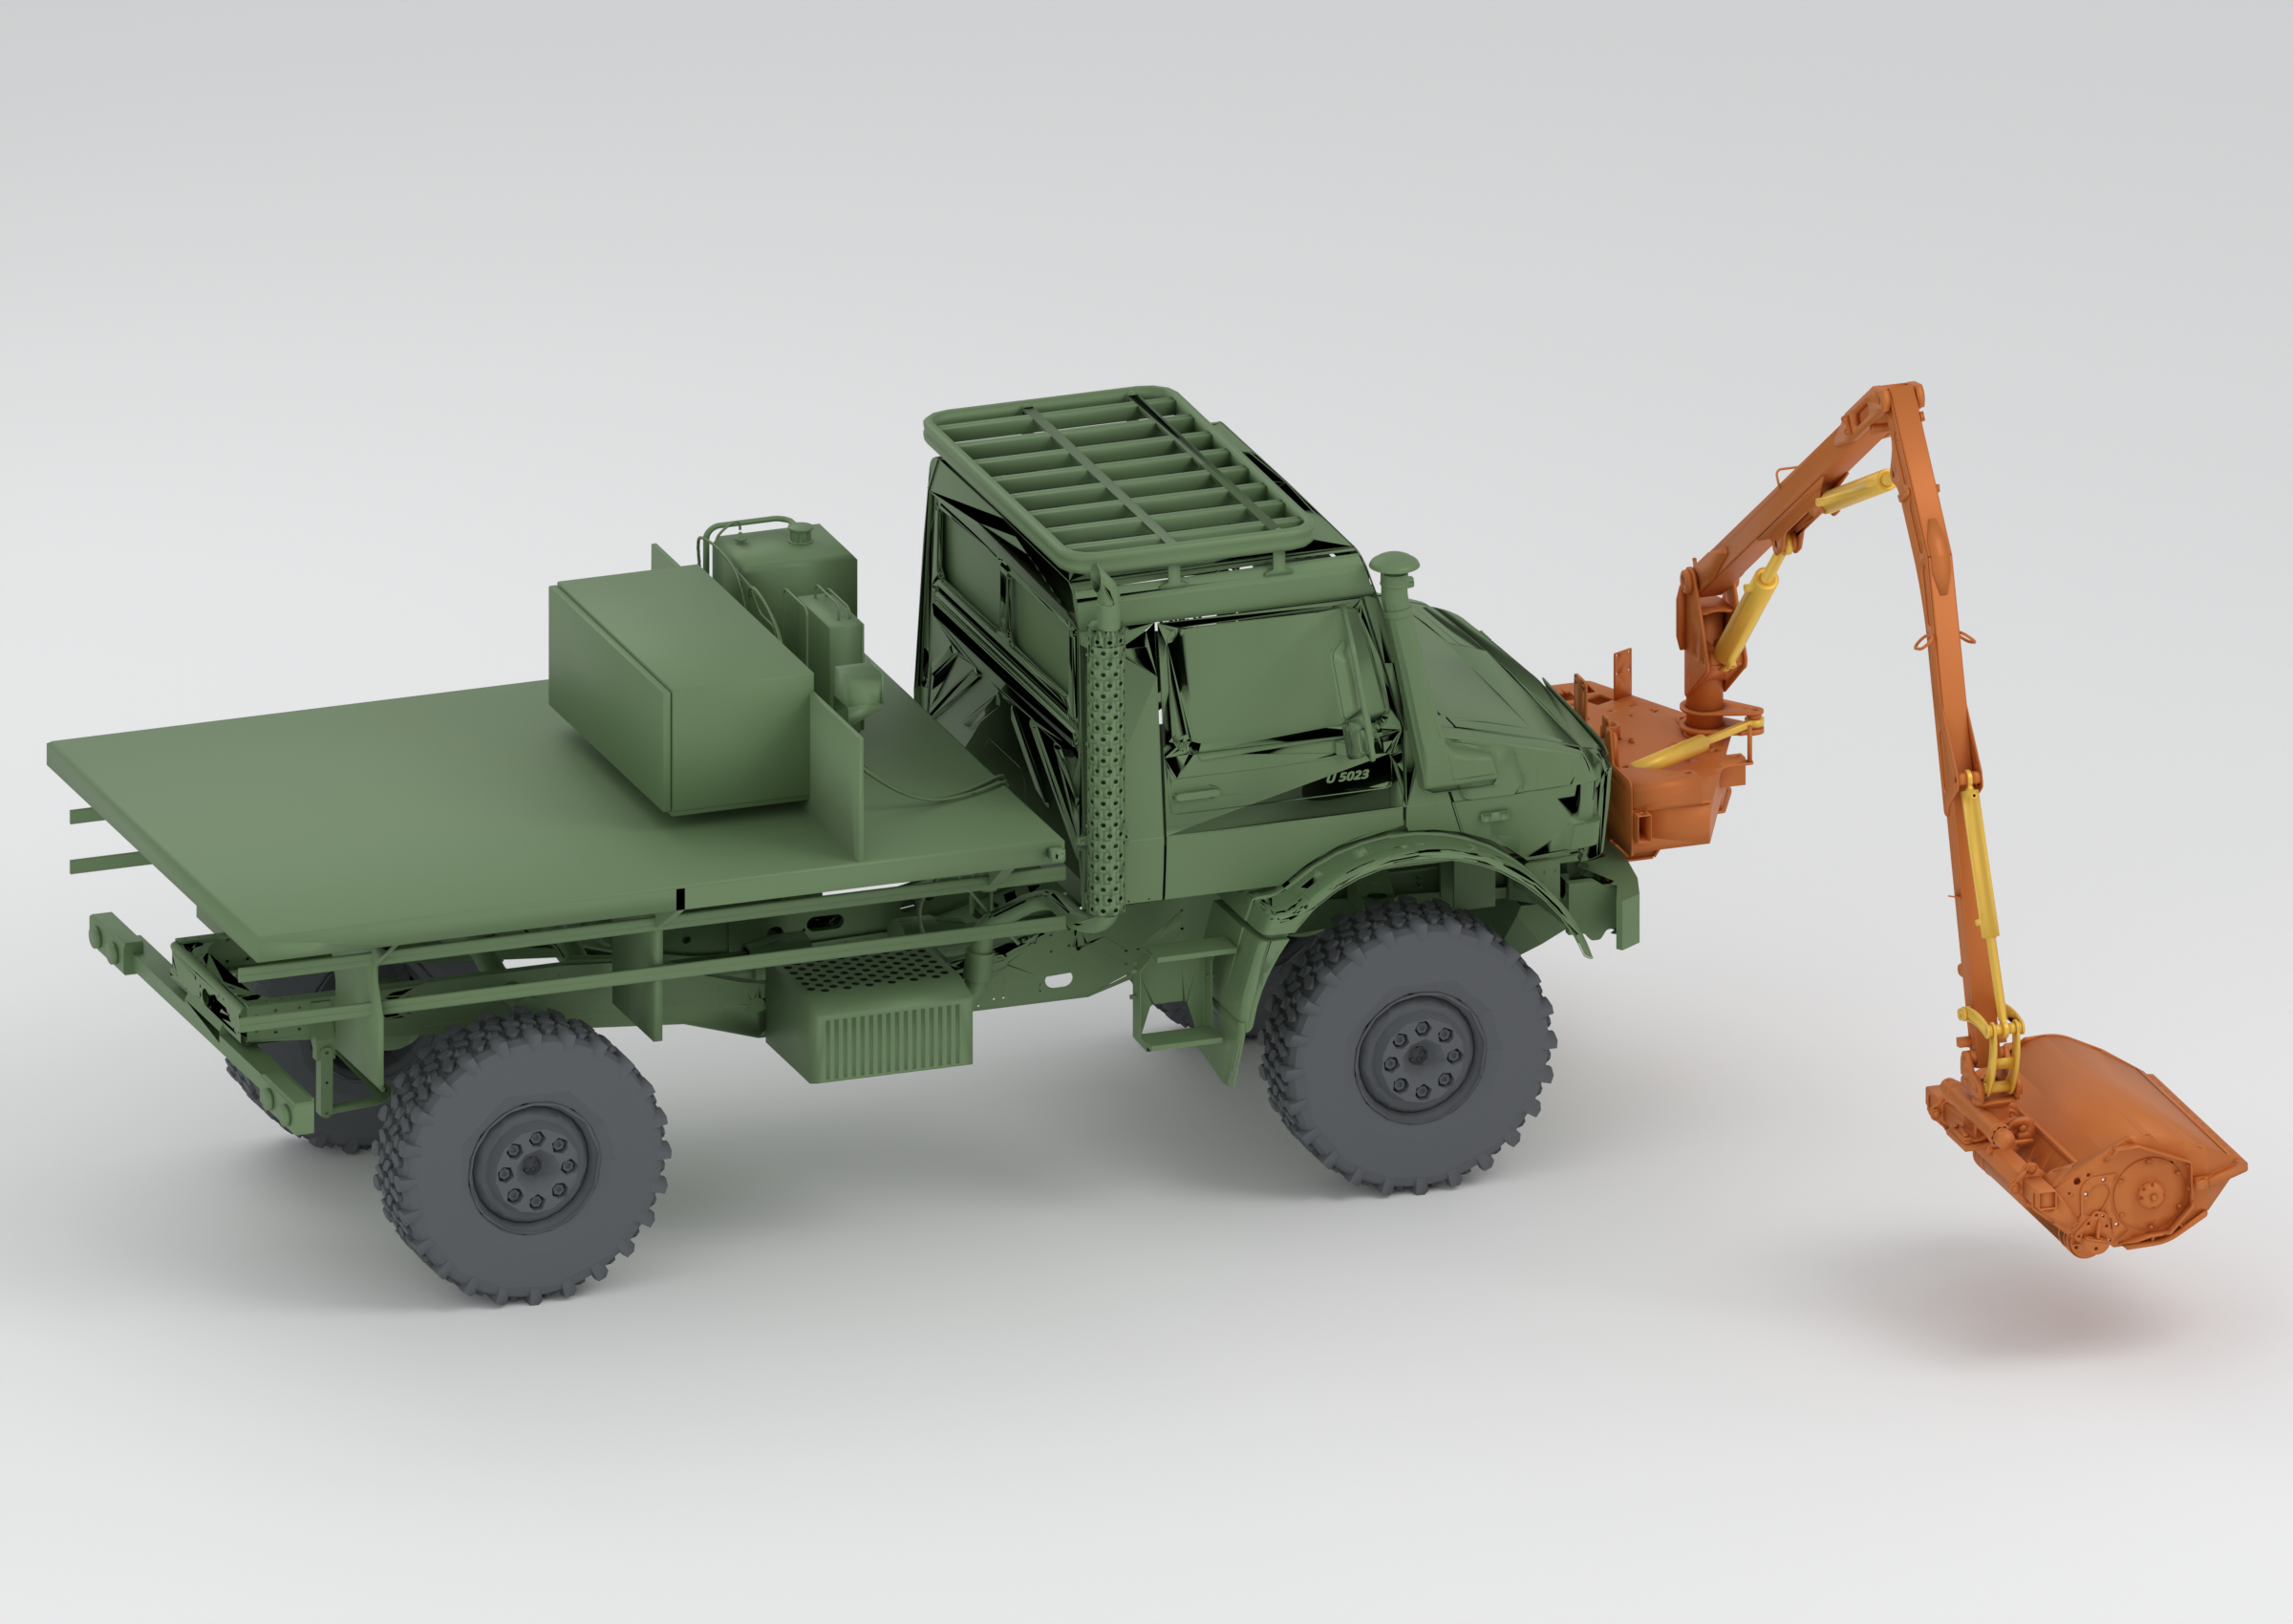
\includegraphics[width=\linewidth]{images/unimog_mulag_rear}
    \caption{}
    \label{fig:sys:unimog-rear}
  \end{subfigure}
  \caption{The complete simulated machine, rendered directly from the
  USD articulation that the IsaacLab environment loads: the Unimog implement carrier with the MULAG FME~500 boom mounted on its front
  frame and the flail head deployed to the side. (a)~Front three-quarter
  view; (b)~rear three-quarter view of the same configuration. The four
  hydraulic cylinders are highlighted in orange, following the
  convention of Figure~\ref{fig:sys:topology}. This is the mechanism, the
  carrier, and the mounting geometry exactly as PhysX simulates them.
  The hydraulics are not present here and enter only through the learned
  actuator models.}
  \label{fig:sys:unimog}
\end{figure}

%% ===== removed 2026-08-13 : fig:sys:bulkmod (bulk-modulus sensitivity) =====
\begin{figure}[tb]
  \centering
  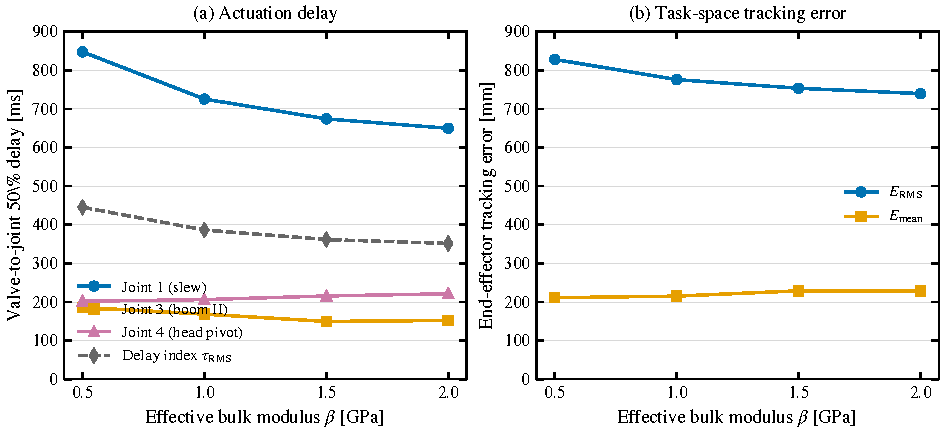
\includegraphics[width=\textwidth]{images/ch3_bulk_modulus_sensitivity}
  \caption{Sensitivity of the Simscape plant to the effective bulk
  modulus, measured in the preceding modeling study.
  (a)~Valve-to-joint 50\,\% delays of
  the dominant axes and the RMS delay index; (b)~end-effector tracking
  error of the fixed validation controller. Softer fluid slows the arm
  and degrades tracking. The effect saturates beyond
  $\unit[1.5]{GPa}$.}
  \label{fig:sys:bulkmod}
\end{figure}
